%!TEX root = ../dokumentation.tex

\chapter{Materialien und Methoden} \label{ch:materialsAndMethods}

Die deutsche Politik in der 19. Legislaturperiode war geprägt von der Bundestagswahl 2017, die als Ausgangspunkt für die politischen Entwicklungen in diesem Zeitraum diente. Die Heterogenität der Parteilandschaft und besondere Ereignisse während dieser Legislaturperiode trugen zur Vielfalt der politischen Strömungen und Dynamiken bei. Die politischen Akteure setzten verschiedene Themenschwerpunkte, um politische Agenden zu gestalten und Herausforderungen anzugehen.

Im Bereich der Textanalyse werden verschiedene Repräsentationsformen von Text wie N-Grams, \ac{BoW}, \ac{TF-IDF}, \ac{GloVe}, \ac{CNN}-Embedding-Schicht, \ft und \ac{BERT} untersucht. Jede Methode hat ihre eigenen Vor- und Nachteile bei der Verarbeitung und Darstellung von Textdaten. Zusätzlich wird ein Modell zur Sentimentanalyse für die deutsche Sprache vorgestellt. Das soll dazu genutzt werden, um die Datensätze in \autoref{ch:crispDm_1} zu analysieren.

\section{Deutsche Politik in der 19. Legislaturperiode}

Dieser Abschnitt gibt ein Überblick über die politische Situation während der \num{19}. Wahlperiode des Deutschen Bundestages. Die politischen Themen und Aussagen spiegeln sich in den zu untersuchenden Texten wider. In \autoref{subsec:btw17} werden der Ausgang und die Folgen der Bundestagswahl \num{2017} beleuchtet und im Anschluss wird in \autoref{subsec:heterogenitätParteien} genauer auf die Parteienlandschaft und parteiinterne Unterschiede und Flügel eingegangen. Schließlich werden in \autoref{subsec:besondereEreignisse} besondere Ereignisse im Untersuchungszeitraum angeführt und in \autoref{subsec:themenschwerpunkte} diejenigen Themen erläutert, die während der Zeit den politischen Diskurs am stärksten geprägt haben.

\subsection{Bundestagswahl \num{2017}} \label{subsec:btw17}

Die Bundestagswahl \num{2017} fand am \num{24}. September \num{2017} statt. \autoref{fig:ergebnisBtw17} zeigt dazu die Aufteilung der Zweitstimmen nach Partei.

\begin{figure}[H]
  \centering
  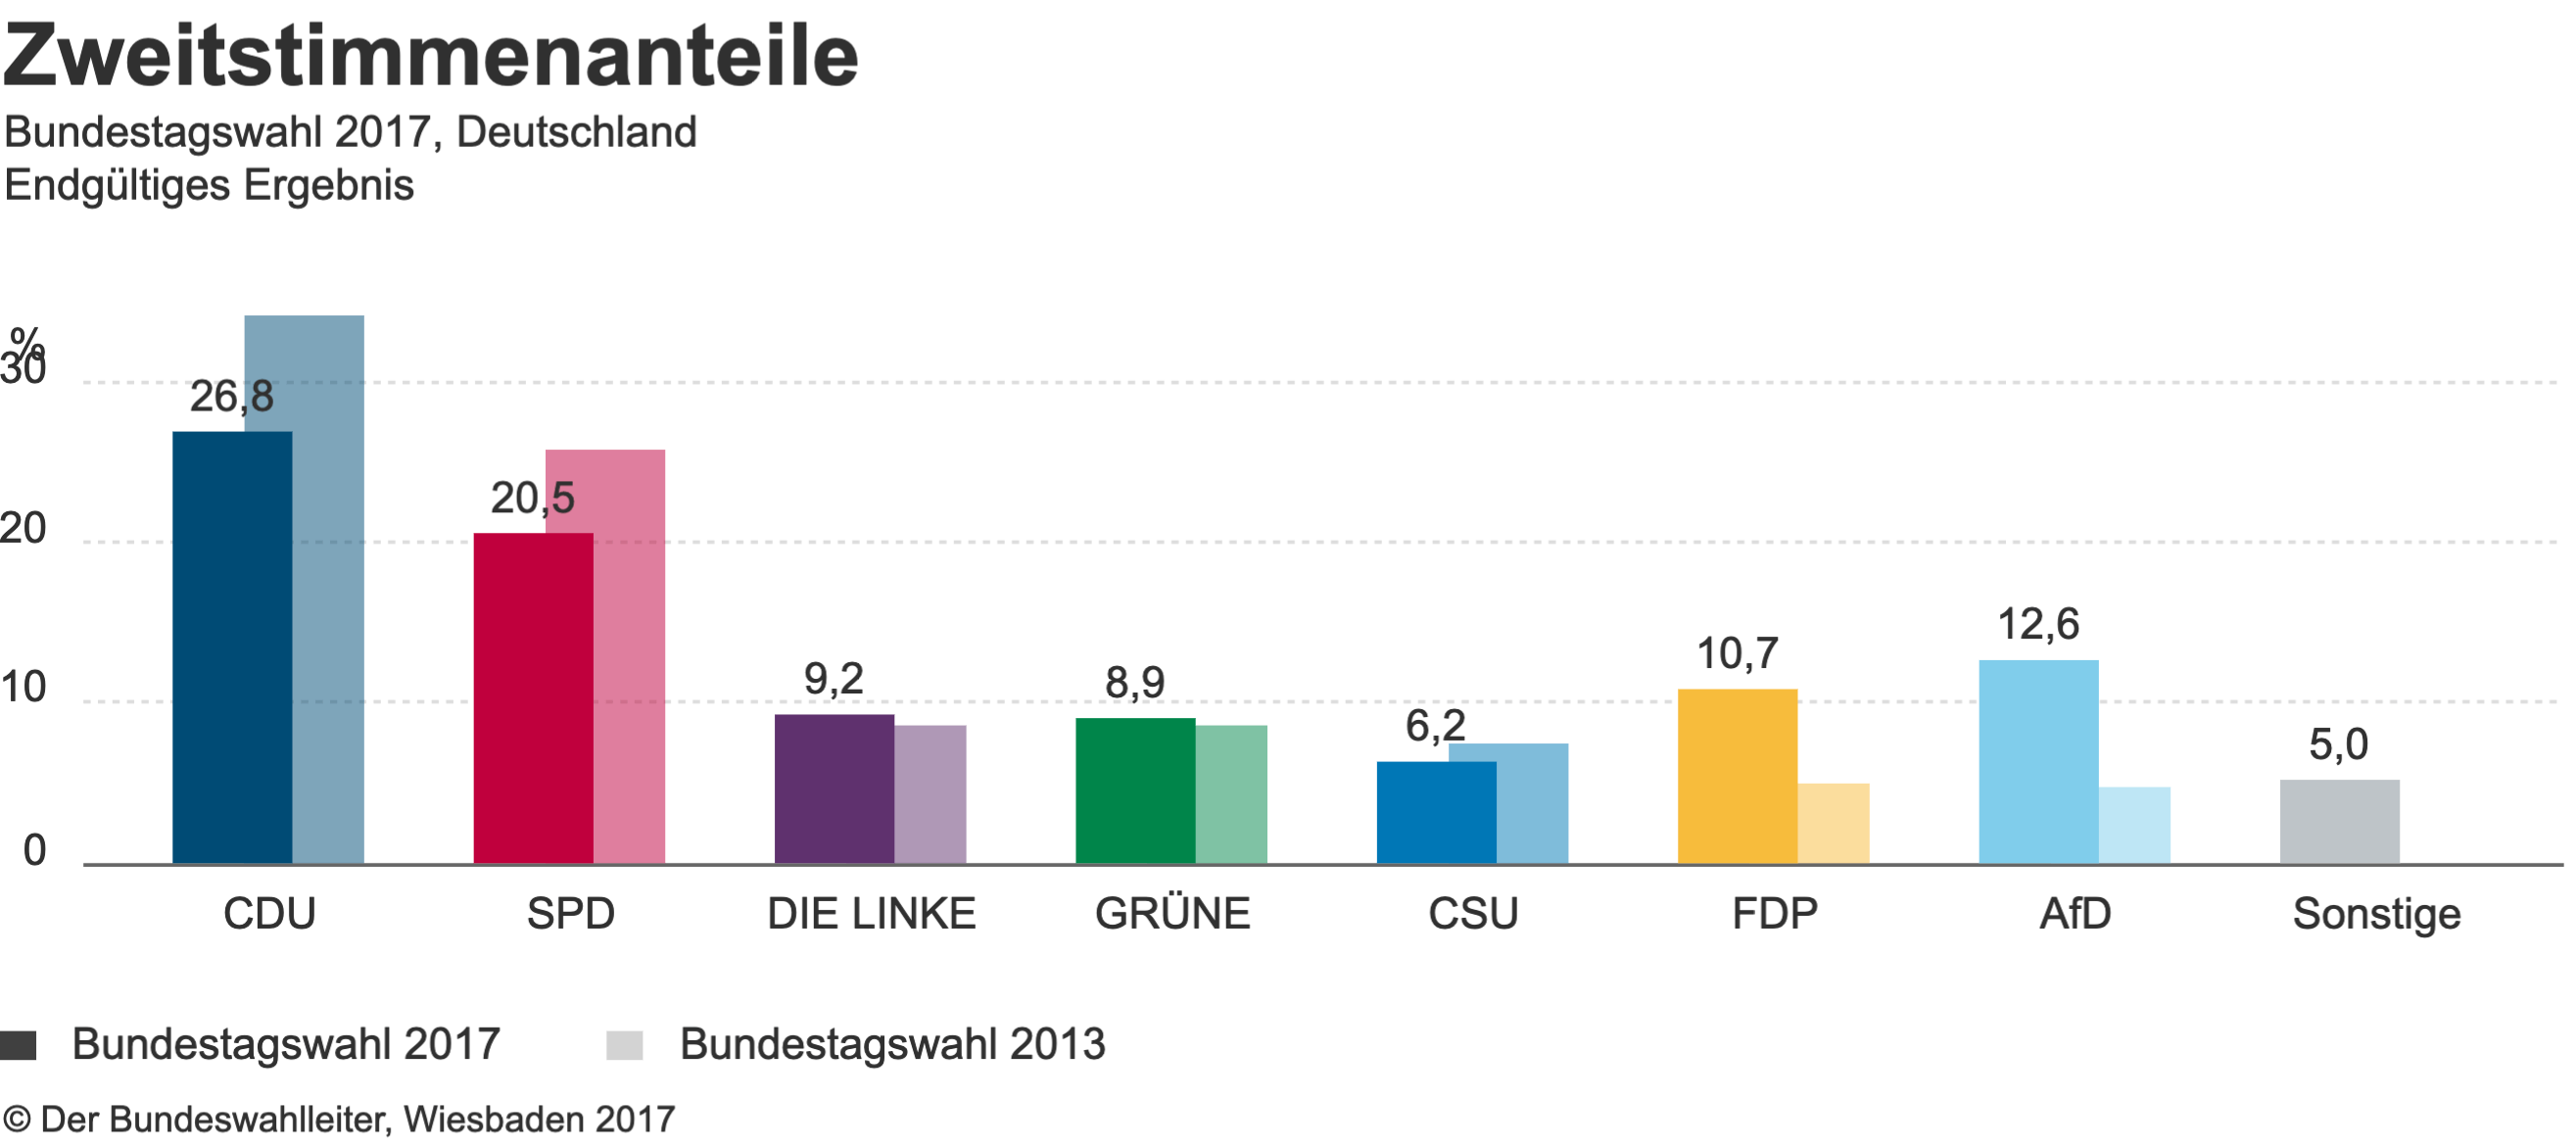
\includegraphics[width=0.9\textwidth]{data/images/ergebnisBtw17.png}
  \caption{Ergebnis der Bundestagswahl \num{2017} \autocite{noauthor_bundestagswahl_nodate}} \label{fig:ergebnisBtw17}
\end{figure}

Die \ac{CDU} erlitt zwar einen starken Verlust bezüglich der vorherigen Wahl, konnte sich aber dennoch mit \SI{26.8}{\percent} der Stimmen als stärkste Kraft durchsetzen. Gemeinsam kommen die \ac{CDU} und \acs{CSU} auf insgesamt \SI{32.9}{\percent}. Die \ac{SPD}, die ebenfalls im Vergleich zur Bundestagswahl \num{2013} an Stimmen verlor, kam auf \SI{20.5}{\percent}. Mit minimalen Steigerungen kamen die Linke auf \SI{9.2}{\percent} und die Grünen auf \SI{8.9}{\percent}. Sowohl die \ac{FDP} mit \SI{10.7}{\percent} als auch die \ac{AfD} mit \SI{12.6}{\percent} konnten ihre Anteile deutlich steigern. Während es die \ac{AfD} durch dieses Ergebnis zum ersten Mal in den Bundestag schaffte, konnte die \ac{FDP} nach dem Ausscheiden \num{2013} erneut in den Bundestag einziehen. Die übrigen Parteien kamen kumuliert auf \SI{5}{\percent} der Stimmen.

Laut \textcite{schmid_deutscher_2021} seien nach der Bundestagswahl \num{2017} zum ersten Mal sieben Parteien und sechs Fraktionen im Bundestag vertreten, was als Zeichen für die weiter abnehmende Bindungskraft der Volksparteien \ac{CDU}, \ac{CSU} und \ac{SPD} gesehen werden kann. Zudem seien besonders die starken Verluste von Union und \ac{SPD} hervorzuheben. Die \ac{SPD} verzeichnete mit der Bundestagswahl außerdem ihr schlechtestes Ergebnis seit \num{1949}.

Im Anschluss an die Wahl begonnen Sondierungsverhandlungen für eine mögliche \enquote{Jamaika-Koalition} zwischen Union, \ac{FDP} und Grünen. Nachdem diese seitens der \ac{FDP} abgebrochen wurden, bildete sich eine Große Koalition aus Union und \ac{SPD}. Damit gab es die längste Regierungsbildung in Deutschland aller Zeiten \parencite{schmid_deutscher_2021}.

\subsection{Heterogenität der Parteienlandschaft} \label{subsec:heterogenitätParteien}

Nach \textcite{niedermayer_entwicklung_2020} weist das deutsche Parteisystem einen Wandel, weg von den alten zwei Volksparteien (\ac{CDU} und \ac{SPD}), hinzu \enquote{einem pluralistischen System an der Grenze zum hochfragmentierten System} auf. Dabei sei besonders bei den Volksparteien ein schrittweiser Verlust der Zustimmung festzustellen, wohingegen sich die Grünen als zweitstärkste Kraft etabliert haben. Zudem habe sich auch die \ac{AfD} fest verankert. Bei der \ac{FDP} und der Linken sei wenig Dynamik zu erkennen.

\textcite{engler_wettbewerb_2022} heben hervor, dass bei vielen Themen die Oppositionsparteien divergente Meinungen entgegen der Regierung und auch untereinander vertreten. Während die Grünen und Linke für konsequentere Klimamaßnahmen plädieren, positioniert sich die \ac{AfD} entgegengesetzt. In der Debatte um Corona-Maßnahmen ergebe sich ein ähnliches Bild, in der sich auch die \ac{FDP} kritisch gegen einige Maßnahmen positioniert habe.

Die politischen Parteien in Deutschland grundlegend in zwei Lager eingeteilt werden: Ein \enquote{links-liberales} bestehend aus \ac{SPD}, Grünen und Linken, sowie ein \enquote{rechts-konservatives} oder \enquote{bürgerliches} bestehend aus der Union und \ac{AfD} \autocite{thomeczek_politische_2019}. Der \ac{FDP} wird als gesellschaftspolitisch liberale, aber wirtschaftspolitisch rechte Partei eine Sonderrolle zugeschrieben. Zudem beobachten \textcite{thomeczek_politische_2019}, dass die Parteien eine unterschiedliche interne Kohärenz aufweisen. Die beiden Volksparteien, \ac{SPD} und \ac{CDU}, weisen dabei durchschnittlich weniger hohe Agreement-Index-Werte -- ein Maßstab, wie stark die Positionen der Mitglieder übereinstimmen -- auf als die anderen Parteien.

Die Verteilung der Positionen innerhalb einer Partei betrachtet auch \textcite{saltzer_bundestagswahl_2022}. \autoref{fig:positionierungAusgewaehlterKanidaten} zeigt die Verortung von Kandidaten für die Bundestagswahl \num{2021} nach Partei. Die x-Achse stellt dabei die Position in der politischen Links-Rechts-Skala und die y-Achse die Zustimmung zu Regierung beziehungsweise Opposition dar.

\begin{figure}[H]
  \centering
  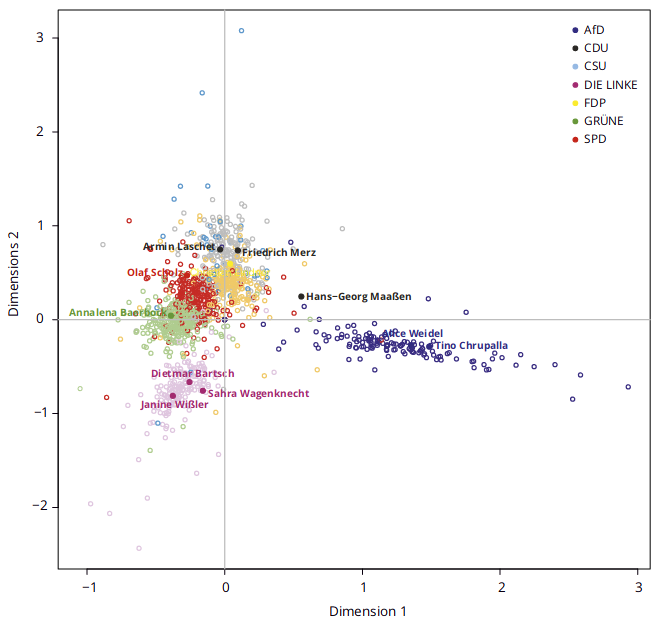
\includegraphics[width=0.5\textwidth]{data/images/positionierung_ausgewaehlter_kandidaten.png}
  \caption[Positionierung ausgewählter Kandidaten \autocite{saltzer_bundestagswahl_2022}]{Positionierung ausgewählter Kandidaten innerhalb eines zweidimensionalen politischen Raums \autocite{saltzer_bundestagswahl_2022}} \label{fig:positionierungAusgewaehlterKanidaten}
\end{figure}

Aus der Grafik geht hervor, dass sich besonders Parteien an den Rändern des politischen Spektrums -- Linke und \ac{AfD} -- von den restlichen Parteien visuell abgrenzen. Die restlichen Parteien verteilen sich rund um den Ursprung des Koordinatensystems herum und überschneiden sich dabei auch.

Kandidaten der Union und \ac{FDP} liegen im Schnitt in der Mitte der Links-Rechts-Skala. Dabei liegt die Regierungs-Zustimmung der Union höher. Im Vergleich zur \ac{FDP} ist die \ac{SPD} weiter links positioniert. Die Kandidaten der Grünen sind noch weiter links eingezeichnet und neutral auf der y-Achse. Die Linke befinden sich ähnlich weit links wie die Grünen, sind aber deutlich eher der Opposition zugeneigt. Die \ac{AfD} ist die einzige Partei, die nach der gegebenen Darstellung rechts der Mitte aufzufinden ist und dabei eher der Opposition nahesteht.

Auffällig ist, dass die Verteilung der \ac{AfD}-Kandidaten auf der Links-Rechts-Skala deutlich stärker verstreut ist im Vergleich zu den anderen Parteien. Eine mögliche Begründung ist der Protest gegen die herkömmlichen Parteien. Daraus ergibt sich eine niedrigere interne Einigkeit zu politischen Themen und eine stärkere Streuung der Meinungen.

\subsection{Besondere Ereignisse im Untersuchungszeitraum} \label{subsec:besondereEreignisse}

\textcite{schmid_deutscher_2021} gibt wichtige öffentlichkeitswirksame Ereignisse während der \num{19}. Wahlperiode des deutschen Bundestages wieder. Darunter fällt zunächst die Corona-Pandemie, der Auswirkungen und der Umgang mit diesen nach den ersten Ansteckungsfällen Anfang 2020 zu einem zentralen Thema in Politik und Gesellschaft wurden. Im Juli 2021 kam es in Teilen von Nordrhein-Westfalen und Rheinland-Pfalz zu einer schweren Flutkatastrophe. Kurz vor Ende der Legislaturperiode wurde zudem der Einsatz der Bundeswehr in Afghanistan beendet, nachdem eine Machtübernahme der Taliban erfolgt war.

Neben der Bundestagswahl \num{2017} fand am 29. Mai 2019 die Wahl des Europäischen Parlaments statt. Zudem wurden in der Periode \num{13} Landtagswahlen ausgerichtet.

\subsection{Themenschwerpunkte} \label{subsec:themenschwerpunkte}

\textcite{engler_wettbewerb_2022} untersuchen die Themenschwerpunkte in politischen Debatten während der \num{19}. Wahlperiode. Anhand von Umfragen der Forschungsgruppe Wahlen ergibt sich folgender Verlauf. Dieser zeigt die Zu- und Abnahme an Relevanz der Themen, die in der Zeitperiode Relevanz hatten.

\begin{figure}[H]
  \centering
  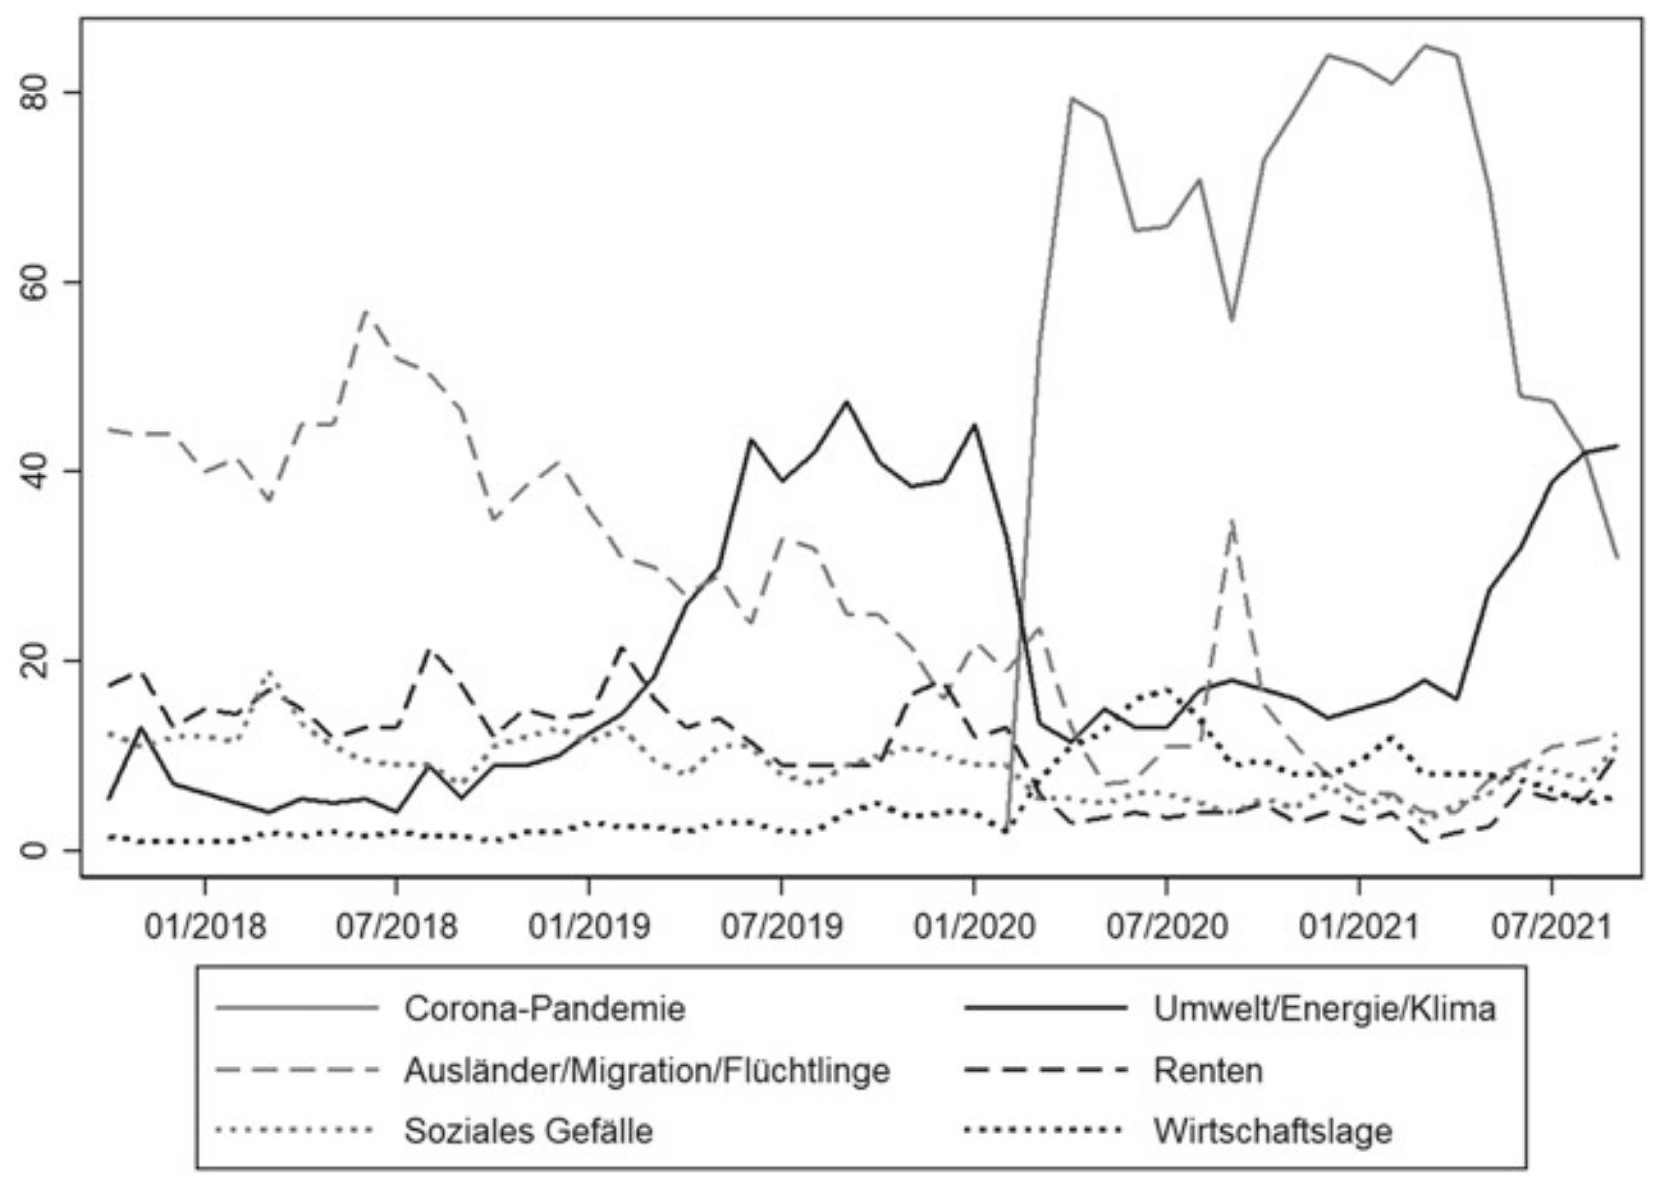
\includegraphics[width=0.8\textwidth]{data/images/themenkonjunktur.png}
  \caption{Verlauf der wichtigsten politischen Themen während der 19. Wahlperiode \autocite{engler_wettbewerb_2022, forschungsgruppe_wahlen_forschungsgruppe_nodate}} \label{fig:themenkonjunktur}
\end{figure}

Zu Beginn der Legislaturperiode war das Thema der Migrationspolitik am wichtigsten. Die Relevanz hat jedoch stetig abgenommen, bis das Thema ab \num{2020} untergeordnet war. Der Themenbereich Umwelt, Energie und Klima wurde ab \num{2019} immer wichtiger und war zeitweise das Thema mit der meisten Relevanz. Nach der Flutkatastrophe \num{2021} wurde diesem Bereich wieder vermehrt Bedeutung zugesprochen. Nach dem Ausbruch der Pandemie war diese schlagartig das mit Abstand dominierende Thema, bis sich die Lage \num{2021} wieder beruhigte. Während des gesamten Zeitraums rückten wirtschafts- und sozialpolitische Themen in den Hintergrund.

Nach \textcite{niedermayer_entwicklung_2020} waren im Betrachtungszeitraum vorwiegend die Flüchtlingskrise sowie das Thema Klimawandel und Energiewende von Bedeutung. Die Dominanz der Klimathematik zeigt sich an Ereignissen wie dem Dieselskandal, der Hitzewelle im Sommer \num{2018} sowie der Popularität der Protestbewegung \enquote{Fridays for Future}.

\section{Repräsentationsformen von Text} \label{sec:representationForms}

Um Analysen und \ac{ML} auf Text anwenden zu können, ist es notwendig diesen in Vektoren umzuwandeln, die durch Maschinen interpretierbar sind. Dafür gibt es unterschiedliche Verfahren, die mitunter den Kontext und komplexe semantische Beziehungen berücksichtigen \autocite{kowsari_text_2019, jurafsky_speech_2023}.

Kontextunabhängige Methoden wie \ac{BoW} und \ac{TF-IDF} extrahieren Informationen über die Häufigkeit einzelner Wörter. \ac{GloVe} ist eine komprimierte Worteinbettungsmethode, die auf der Basis von Kookkurrenzstatistiken und der Verteilung der Wörter im Korpus beruht. Mit diesen Verfahren lässt sich meist nur rudimentär die Semantik eines Satzes abbilden, da jegliche Informationen über den aktuellen Kontext fehlt. Ein alternativer Ansatz ist die Repräsentation mittels kontextabhängigen Verfahren. Neuronale Netze, unter anderem \ac{LSTM}-Netzwerke und Transformer-basierte Modelle, können Zusammenhänge innerhalb eines Satzes erkennen. \ft berücksichtigt Subwort-Informationen, weswegen es kontextabhängig ist. Außerdem ermöglicht es einfache semantische Zusammenhänge abzubilden.

Worteinbettungen (engl. Word Embeddings) spielen eine zentrale Rolle bei der Analyse und dem Training von \ac{NLP}-Modellen. Diese bilden einzigartige Wörter mittels mehrdimensionalen Vektoren\footnote{Häufig bestehen Word Embeddings aus \num{300} Dimensionen} ab. Abhängig vom Verfahren sind die resultierenden Vektoren komprimiert oder unkomprimiert. Worteinbettungen ermöglichen es, Wörter mit einer ähnlichen Bedeutung im mehrdimensionalen Raum zu gruppieren.

Die unterschiedlichen Verfahren können auf Wort-, Satz- oder Dokumentebene angewendet werden.

\subsection*{N-Gram}

N-Grams sind die Grundlage für Verfahren wie \ac{BoW} und \ft. Bei dieser Methode werden Zeichen (Wortebene) oder Wörter (Satzebene) in Fragmente mit der Länge \texttt{n} unterteilt \autocite[5]{kowsari_text_2019}. Die Reihenfolge der Elemente bleibt dabei unverändert.

\subsection*{\acl{BoW}}

\ac{BoW} ist eine simple Repräsentationsform, die lediglich die Häufigkeit von einzigartigen Wörtern berechnet \autocite[6]{kowsari_text_2019}. Im ersten Schritt des Verfahrens, wird ein Satz oder Dokument in eine Menge an 1-Grams (einzelne Wörter) transformiert. Anschließend wird die Liste auf die einzigartigen Wörter reduziert und gezählt, wie häufig die einzigartigen Wörter (engl. Features) auftreten. Die daraus entstehende Tabelle wird auch \ac{BoF} genannt.

Um zu demonstrieren, wie \ac{BoW} funktioniert, nennt \textcite[6]{kowsari_text_2019} folgendes Beispiel: \enquote{As the home to UVA’s recognized undergraduate and graduate degree programs in systems engineering. In the UVA Department of Systems and Information Engineering, our students are exposed to a wide range of range.} Aus dem Text resultiert die folgende \ac{BoF}-Tabelle: \enquote{\{1,1,1,3,2,1,2,1,2,3,1,1,1,2,1,1,1,1,1,1\}}.

Aufgrund von fehlendem syntaktischem Verständnis lässt sich zum Beispiel mit \ac{BoW} nicht zwischen \textit{\enquote{Das ist gut}} und \textit{\enquote{Ist das gut}} unterscheiden \autocite[6]{kowsari_text_2019}.

\subsection*{\acl{TF-IDF}}

Neben der reinen Häufigkeit berücksichtigt \ac{TF-IDF} außerdem die Häufigkeit eines Wortes für eine Sammlung an Dokumenten \autocite[7]{kowsari_text_2019}. Damit ist es möglich, Wörter aus Wortgruppen wie Artikeln, Präpositionen, Konjunktionen von relevanten Wörtern (meist Adjektive, Verben und Nomen) zu trennen.

\[\mathrm{tfidf}(t,d,D) = \frac{f_{t,d}}{{\sum_{t' \in d}{f_{t',d}}}} \cdot \log \frac{N}{|\{d \in D: t \in d\}|}\]

Dafür wird zunächst die relative oder absolute Häufigkeit eines Wortes innerhalb eines Dokumentes berechnet. Außerdem wird die Häufigkeit in anderen Dokumenten berechnet. Der sich daraus ergebene Wert gibt Auskunft darüber, ob es sich um ein generell häufiges Wort oder nicht handelt.

\subsection*{GloVe}

\ac{GloVe} repräsentiert jedes Wort durch ein hochdimensionaler Vektor \autocite[8\psq]{kowsari_text_2019}. Aufgrund der großen Menge an benötigten Daten zum Trainieren, ist es üblich, vortrainierte Worteinbettungen zu verwenden. Laut \citeauthor{kowsari_text_2019} werden hierfür Datensätze wie Wikipedia und Gigaword \num{5} verwendet. Die erzeugten Worteinbettungen sind anschließend in der Lage, mittels der Euklidischen Distanz sprachliche oder semantische Ähnlichkeiten festzustellen \autocite{pennington_glove_2014}. Zusätzlich weisen die Wortvektoren lineare Unterstrukturen auf.

\begin{figure}[H]
  \centering
  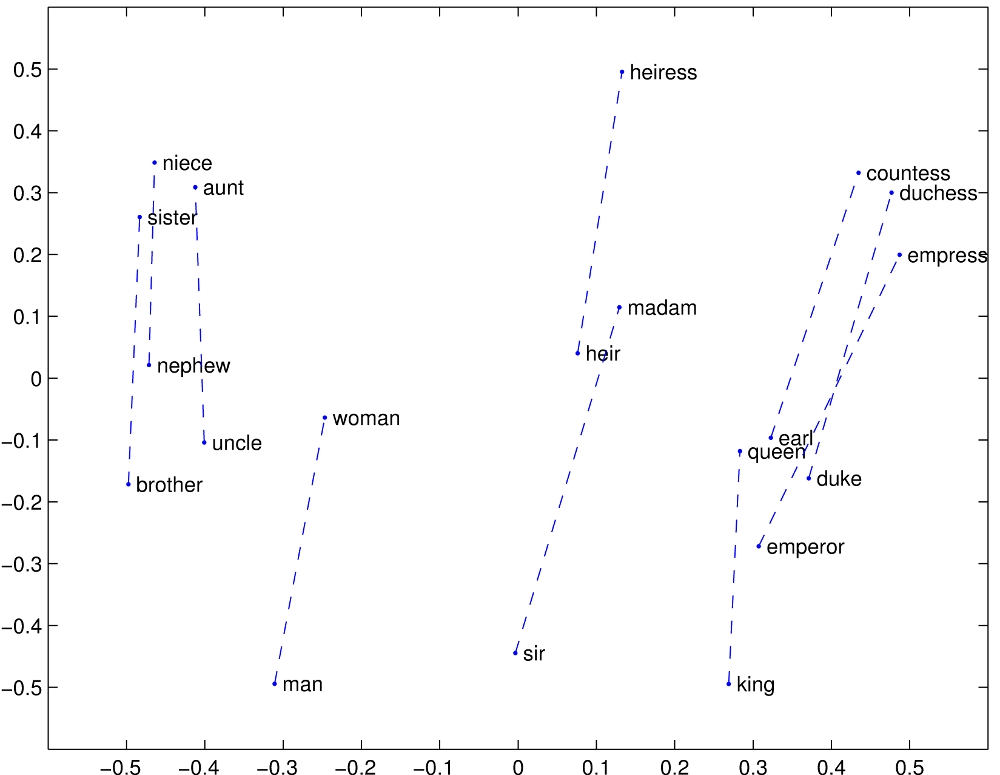
\includegraphics[width=0.6\textwidth]{data/images/materials_and_methods/man_woman.jpg}
  \caption{Mann - Frau Beispiel \acs{GloVe} \autocite{pennington_glove_2014}} \label{fig:gloveExample}
\end{figure}

Das in \autoref{fig:gloveExample} gezeigte Beispiel ist eine der am häufigsten verwendeten Veranschaulichungen von \ac{GloVe}. Die Grafik zeig diverse Wörter in einem zweidimensionalen Raum. Auf dieser Basis der linearen Unterstrukturen lassen sich Wörter addieren und subtrahieren. So zum Beispiel ergibt sich aus \(king - man + woman = queen\). Negativ anzumerken ist jedoch, dass \ac{GloVe} ausschließlich auf Wörtern funktioniert, auf den es auch trainiert wurde.

\subsection*{Embedding-Schicht in neuronalen Netzwerken}

Um Worteinbettungen in neuronalen Netzwerken zu nutzen, muss eine Embedding-Schicht den Eingabetext in eine Sequenz von Wortvektoren umwandeln. Diesen Prozess stellt \autoref{fig:embeddingLayer} dar.

\begin{figure}[H]
  \centering
  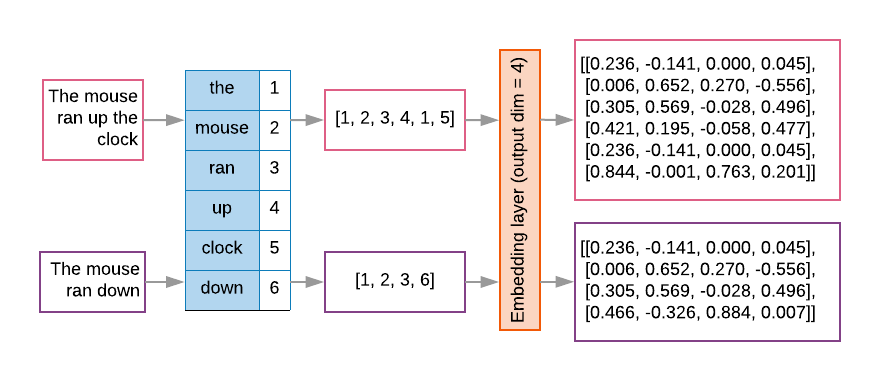
\includegraphics[width=0.8\textwidth]{data/images/embedding_layer.png}
  \caption{Funktionsweise der Embedding-Schicht \autocite{google_prepare_2022}} \label{fig:embeddingLayer}
\end{figure}

Zunächst muss ein Wort-Index basierend auf allen Trainings-Texten erstellt werden, der jedem im Datensatz vorkommenden Wort einen eindeutigen Index zuweist. Mit diesem kann jeder Text in eine Abfolge von Indices umgewandelt werden. In der Embedding-Schicht wird jeder Index durch den Vektor, der das entsprechende Wort darstellt, ersetzt. Die Länge des Vektors ist abhängig davon, welche Dimensionen die Worteinbettungen bereitstellen. Als Endresultat entsteht pro Text eine Liste aus den Wordvektoren für jedes Wort in dem Eingabetext, die an die weiteren Schichten des Netzes weitergegeben wird.

\subsection*{fastText}

Anstelle von ganzen Wörtern, verwendet \ft zum Trainieren und Klassifizieren n-grams bestehend aus \textit{n} Zeichen \autocite{kowsari_text_2019, joulin_fasttextzip_2016}. Ein Beispiel ist das Wort \textit{Tischtennis}, das mit \(n = 3\) in \textit{<Ti,Tis,isc,sch,cht,hte,ten,enn,nni,nis,is>} zerlegt wird. Wörter, die in ähnliche n-grams zerlegt werden können, resultieren in Vektoren, die nah im Vektorraum beieinanderliegen. Die Optimierung während des Trainings und Klassifikation erfolgt mittels der Softmax-Funktion. Zusätzlich wird bag-of-n-grams genutzt, um Zusammenhänge in einem Text zu erkennen \autocite[2]{joulin_bag_2016}. Aufgrund der n-gram Methodik und der niedrigen Komplexität von \(O(h \log_{2}(k))\) des Optimierungs- und Klassifikationsverfahren, eignet sich \ft für die Klassifikation von großen Mengen an Text \autocite[2\psqq]{joulin_bag_2016}.

Im Vergleich zu \ac{GloVe} lassen sich mittels \ft auch Wörter klassifizieren, die im Datensatz enthalten sind \autocite{guhr_training_2020, bojanowski_enriching_2017}. Das ist besonders bei komplexen Sprachen wie Deutsch, die zusammengesetzte Wörter verwenden, hilfreich. Ein Beispiel ist das Wort Tischtennis, das im Englischen \textit{table tennis} lautet.

\subsection*{BERT}

Bei \ac{BERT} handelt es sich um ein tiefes neuronales Netz. Das Modell beruht auf der Transformer-Architektur \autocite[3]{devlin_bert_2019}. Durch den bidirektionalen Ansatz ist es möglich, deutlich besser den Kontext eines Satzes zu verstehen. Das liegt daran, dass vorherige Modelle ausschließlich von vorn nach hinten oder umgekehrt einen Satz verarbeiten konnten. \ac{BERT} hingegen verarbeitet den gesamten Satz auf einmal. Im Trainingsprozess werden zufällig Wörter maskiert \autocite[4]{devlin_bert_2019}. Die Autoren beschreiben außerdem, dass das Modell den nächsten Satz vorhersagt und abgleicht. Beide Methoden helfen dabei, gezielt Eigenschaften der Trainingsdaten zu erlernen.

Neben englischsprachigen Modellen lassen sich ebenfalls deutsche finden. Weiterhin existieren reduzierte Modelle, wie DistilBERT, die weniger Ressourcen benötigten ohne größere Performance-Einbußen.

\section{Sentimentanalyse} \label{sec:sentimentanalysis}

Herkömmliche Methoden zur Bestimmung des Sentiments von deutschen Texten sind Sentiment-Wörterbücher und \ac{ML}-Modellen wie \ac{SVM}, \ac{CNN} und \ac{LSTM} \autocite[1627\psq]{guhr_training_2020}. Alle genannten Methoden erreichen einen $F_1$ Score von \numrange{46.5}{74.9}.

Die Arbeit von \textcite{guhr_training_2020} zeigt, wie sich Texte anhand ihres Sentiments -- positiv, neutral, oder negativ -- durch \ac{BERT} klassifizieren lassen. Für das Training nutzen die Autoren acht unterschiedliche Datensätze, die insgesamt \num{5.3} Millionen Einträge umfassen. Neben einem \ac{BERT}-Modell wurde ebenfalls ein Modell mittels \ft trainiert. Dieses erreicht jedoch einen leicht schlechteren $F_1$ Score\footnote{Mit dem unbalancierten Datensatz erreicht \ac{BERT} einen $F_1$ Score von \num{97.44} und \ft \num{95.73}. Bei dem balanciertem Datensatz erreicht \ac{BERT} einen $F_1$ Score von \num{96.36} und \ft \num{94.05}.} als das \ac{BERT}-Modell \autocite[\psq 1630]{guhr_training_2020}.

Auffällig ist, dass das Modell einen signifikant schlechteren $F_1$ Score erreichen, wenn der Datensatz Tweets oder andere Social Media Posts inkludiert. Das zeigt sich bei den Datensätzen PlotTS, SB10k und GermEval-2017. Bei der Klassifikation dieser erreicht das Modell lediglich einen $F_1$ Score von \numrange{0.6423}{0.7885} \autocite[1631]{guhr_training_2020}.

\section{Zusammenfassung}

Im ersten Abschnitt des Kapitels wird die politische Situation in Deutschland zur Zeit der \num{19}. Legislaturperiode skizziert. Die Volksparteien \ac{CDU}/\ac{CSU} und \ac{SPD} haben bei der Bundestagswahl \num{2017} Verluste hinnehmen müssen, bilden jedoch eine Große Koalition. Die Grünen und die \ac{AfD} erleben einen Aufschwung und sorgen so dafür, dass das Parteiensystem diverser wird. Im Untersuchungszeitraum bestimmten hauptsächlich die Themenbereiche Migration, Klimaschutz und Pandemie den Diskurs.

Der zweite Abschnitt des Kapitels umreißt die Basismethoden zur Analyse und Klassifizierung von Texten. \ac{BoW} und \ac{TF-IDF} sind die beiden einfachsten Methoden, die lediglich die Häufigkeit einzigartiger Wörter betrachten. \ac{BoW} betrachtet dabei ein einzelnes Dokument, während \ac{TF-IDF} auch die Häufigkeit über mehrere Dokumente hinweg berücksichtigt. Im Gegensatz zu diesen beiden unkomprimierten Verfahren nutzen Word2Vec, GloVe und \ft komprimierte Vektoren, die Wörter oder Zeichen basierend auf ihrem Kontext einem Vektor im Vektorraum zuordnen.

Für die Analyse mittels deskriptiver Statistik in \autoref{ch:crispDm_1} wird ein Modell zur Bestimmung der Stimmung eines Textes betrachtet. Dieses Modell liefert Aufschluss darüber, ob ein Text positiv, negativ oder neutral klingt.
